\documentclass[a4paper,10pt]{article}

\usepackage{amsmath}
\usepackage[utf8]{inputenc} % pour les accents
\usepackage[T1]{fontenc} % caracteres francais
\usepackage{geometry} %les marges
\usepackage[french]{babel} %langue principale
\usepackage[dvips]{graphicx}
\geometry{ hmargin=2cm, vmargin=2cm }

\pagestyle{empty} %pas de numerotation de page

%
% Debut du document
%
\begin{document}

\section*{FICHE DE VALIDATION DU LOGICIEL MASCARET V7P0}

\subsection*{Validation du noyau transcritique}

\subsection*{\emph{Ecoulement permanent dans l'Oriège}}

\subsection*{Numéro du cas test : 19}

\subsection*{Auteur : Fabrice ZAOUI}


\vspace{1cm}

\subsection*{Description}

Le cas test consiste à modéliser la vallée de l'Oriège sur $5\ km$ en aval de l'usine d'Orlu. Il s'agit de réaliser un modèle hydraulique de la vallée de l'Oriège
pour la propagation d'éclusées. Des mesures en régime permanent ont été faites pour caler le modèle.

Cette étude est particulièrement intéressante car elle permet de valider le schéma sur un cas réel d'écoulement permanent dans un torrent avec toutes les difficultés (écoulement torrentiel avec de très faibles débits, forte pente ($5\%$), présence de vasques) qu'implique ce type d'écoulement.

\subsection*{Données géométriques}

La vallée de l'Oriège ($5\ km$ de longueur) est modélisée par $75$ profils en travers. Ces profils levés par le LNHE ont été placés, dans la mesure du possible, de manière à représenter correctement la géométrie moyenne de la rivière. Certaines zones n'ont pas fait l'objet de relevés bathymétriques par manque d'accessibilité. De plus, $13$ échelles limnimétriques ont été implantées afin de réaliser des lignes d'eau à débit permanent. Ces mesures nous serviront pour la validation du modèle. Plus de renseignements sur ce modèle sont disponibles\footnote{E. Demay, \emph{Eclusées de l'Oriège. Bilan des travaux effectués en 1993 par le LNH}, Rapport EDF HE-43/93.43}.

\subsection*{Données physiques}

\begin{itemize}
 \item Débit amont de $12.36\ m^3/s$ avec un apport de $0.85\ m^3/s$ en $x = 2938\ m$;
 \item Conditions aux limites :
 \begin{itemize}
  \item Débit imposé à l'amont correspondant au débit permanent recherché;
  \item Cote imposée à l'aval. 
 \end{itemize}
 \item Conditions initiales : ligne d'eau permanente calculée par le code SARAP.
\end{itemize}

\subsection*{Données numériques}

\begin{itemize}
 \item Pas de temps variable déterminé par un nombre de Corant égal à 0.8;
 \item Durée de la simulation jusqu'à obtenir un débit permanent : $8000$ pas de temps;
 \item Modélisation explicite du frottement;
 \item Pas de planimétrage de $0.3$;
 \item Maillage avec un pas d'espace variable :
 \begin{itemize}
  \item $29$ mailles pour $0\ m \leq x \leq 200\ m$;
  \item $350$ mailles pour $200\ m < x \leq 1500\ m$;
  \item $550$ mailles pour $1500\ m < x \leq 5043\ m$.
 \end{itemize}

\end{itemize}

\subsection*{Résultats}

Sur les figures~\ref{fig1} et \ref{fig2}, sont représentés le débit permanent et la cote. On remarque que le débit permanent calculé présente peu d'oscillations et ces dernières atteignent $10\%$ d'amplitude. Les oscillations correspondent aux zones à forte variation du nombre de Froude. Le nouyau permanent ne présente pas d'oscillation dans ses résultats.

Sur le tableau~\ref{tab1}, sont comparées les cotes calculées et les mesures. On note un bon accord entre les mesures et le calcul.

Le noyau Permanent du logiciel Mascaret $7.0$ permet à présent de traiter les régimes torrentiels. La figure~\ref{fig3} compare les résultats des hauteurs d'eau obtenues
avec ce code, elles sont quasi identiques. La figure~\ref{fig4} donne une comparaison des nombres de Froude obtenus avec les deux noyaux, ils sont là-aussi similaires.



\begin{center}
 \begin{table}
 \caption{Cotes mesurées et calculées}
 \label{tab1}
 \centering
 \begin{tabular}{|c|c|c|c|}
  \hline
  Abscisses ($m$) & Cote mesurée ($m$) & cote calculée ($m$) & Ecarts ($m$) \\
  \hline \hline
  0 & 899.89 & 899.66 & -0.23 \\
  340 & 893.62 & 893.66 & 0.04 \\
  564.5 & 883.76 & 883.64 & -0.12 \\
  1594 & 864.91 & 864.67 & -0.24 \\
  2119 & 846.99 & 846.62 & -0.37 \\
  2132.5 & 845.69 & 845.81 & 0.12 \\
  2402.5 & 838.6 & 838.54 & -0.06 \\
  2716.5 & 835.33 & 835.18 & -0.15 \\
  3216.5 & 830.05 & 830.1 & 0.05 \\
  3829.5 & 825.59 & 825.52 & -0.07 \\
  4354 & 821.94 & 821.96 & 0.02 \\
  4442 & 821.15 & 821.25 & 0.1 \\
  5007 & 817.4 & 817.61 & 0.21 \\
  \hline
 \end{tabular}
 \end{table}
\end{center}

\newpage
~

\begin{figure}
 \begin{center}
  \includegraphics[angle=270,width=15cm]{Qconv.eps}
  \caption{Débit résultat}
  \label{fig1}
 \end{center}
\end{figure}

\begin{figure}
 \begin{center}
  \includegraphics[angle=270,width=15cm]{Zconv.eps}
  \caption{Ligne d'eau convergée}
  \label{fig2}
 \end{center}
\end{figure}

\begin{figure}
 \begin{center}
  \includegraphics[angle=270,width=15cm]{H_Tr_Pr.eps}
  \caption{Hauteurs d'eau comparées}
  \label{fig3}
 \end{center}
\end{figure}

\begin{figure}
 \begin{center}
  \includegraphics[angle=270,width=15cm]{Froude_Tr_Pr.eps}
  \caption{nombre de Froude comparés}
  \label{fig4}
 \end{center}
\end{figure}

%
% fin du document
%
\end{document}          
